\subsection{Trajectory - Thomas Satterly}

\subsubsection{Physics Integration Model}
The trajectory of the boosted stack and SFRJ is a natural fallout of the physics model interacting with attitude controllers and the calculated lift, drag, thrust, and gravity forces. A three-degrees-of-freedom point mass model was used in conjunction with a Runge-Kutta 4th order integrator, described in Equations \ref{eqn:RK4_1} - \ref{eqn:RK4_6} for simulating linear motion. The orientation vector, which is decoupled from the velocity vector out of a necessity to simulate pitch, roll, and yaw maneuvers, was handled outside of the physics integration by assuming constant turn rates for simplicity. 

\begin{align}
    y_{n+1} &= y_n + \frac{1}{6}(k_1 + 2k_2 + 2k_3 + k_4) 
    \label{eqn:RK4_1} \\
    t_{n+1} &= t_n + h 
    \label{eqn:RK4_2}\\
    k_1 &= hf(t_n, y_n) 
    \label{eqn:RK4_3}\\
    k_2 &= hf(t_n + \frac{h}{2}, y_n + \frac{k_1}{2}) 
    \label{eqn:RK4_4}\\
    k_3 &= hf(t_n + \frac{h}{2}, y_n + \frac{k_2}{2}) 
    \label{eqn:RK4_5}\\
    k_4 &= hf(t_n + h, y_n + k_3)
    \label{eqn:RK4_6}
\end{align}
\begin{align*}
y_n&: \text{Vehicle state}\\
t_n&: \text{Time}\\
h&: \text{Change in time}\\
f(t_n, y_n)&: \text{Change of state as a function of time and state}
\end{align*}

A time step convergence study was conducted by simulating a Cesaroni Pro150-40k 40960O8000-P boosting a small secondary stage that, once dropped at boost stage burnout, burns for and additional 5 seconds. The altitude and speed of the second stage was recorded and compared after 30 seconds of total simulation time. The results are shown in Figure \ref{fig:timeStepConvergence}.

\begin{figure}[H]
\centering
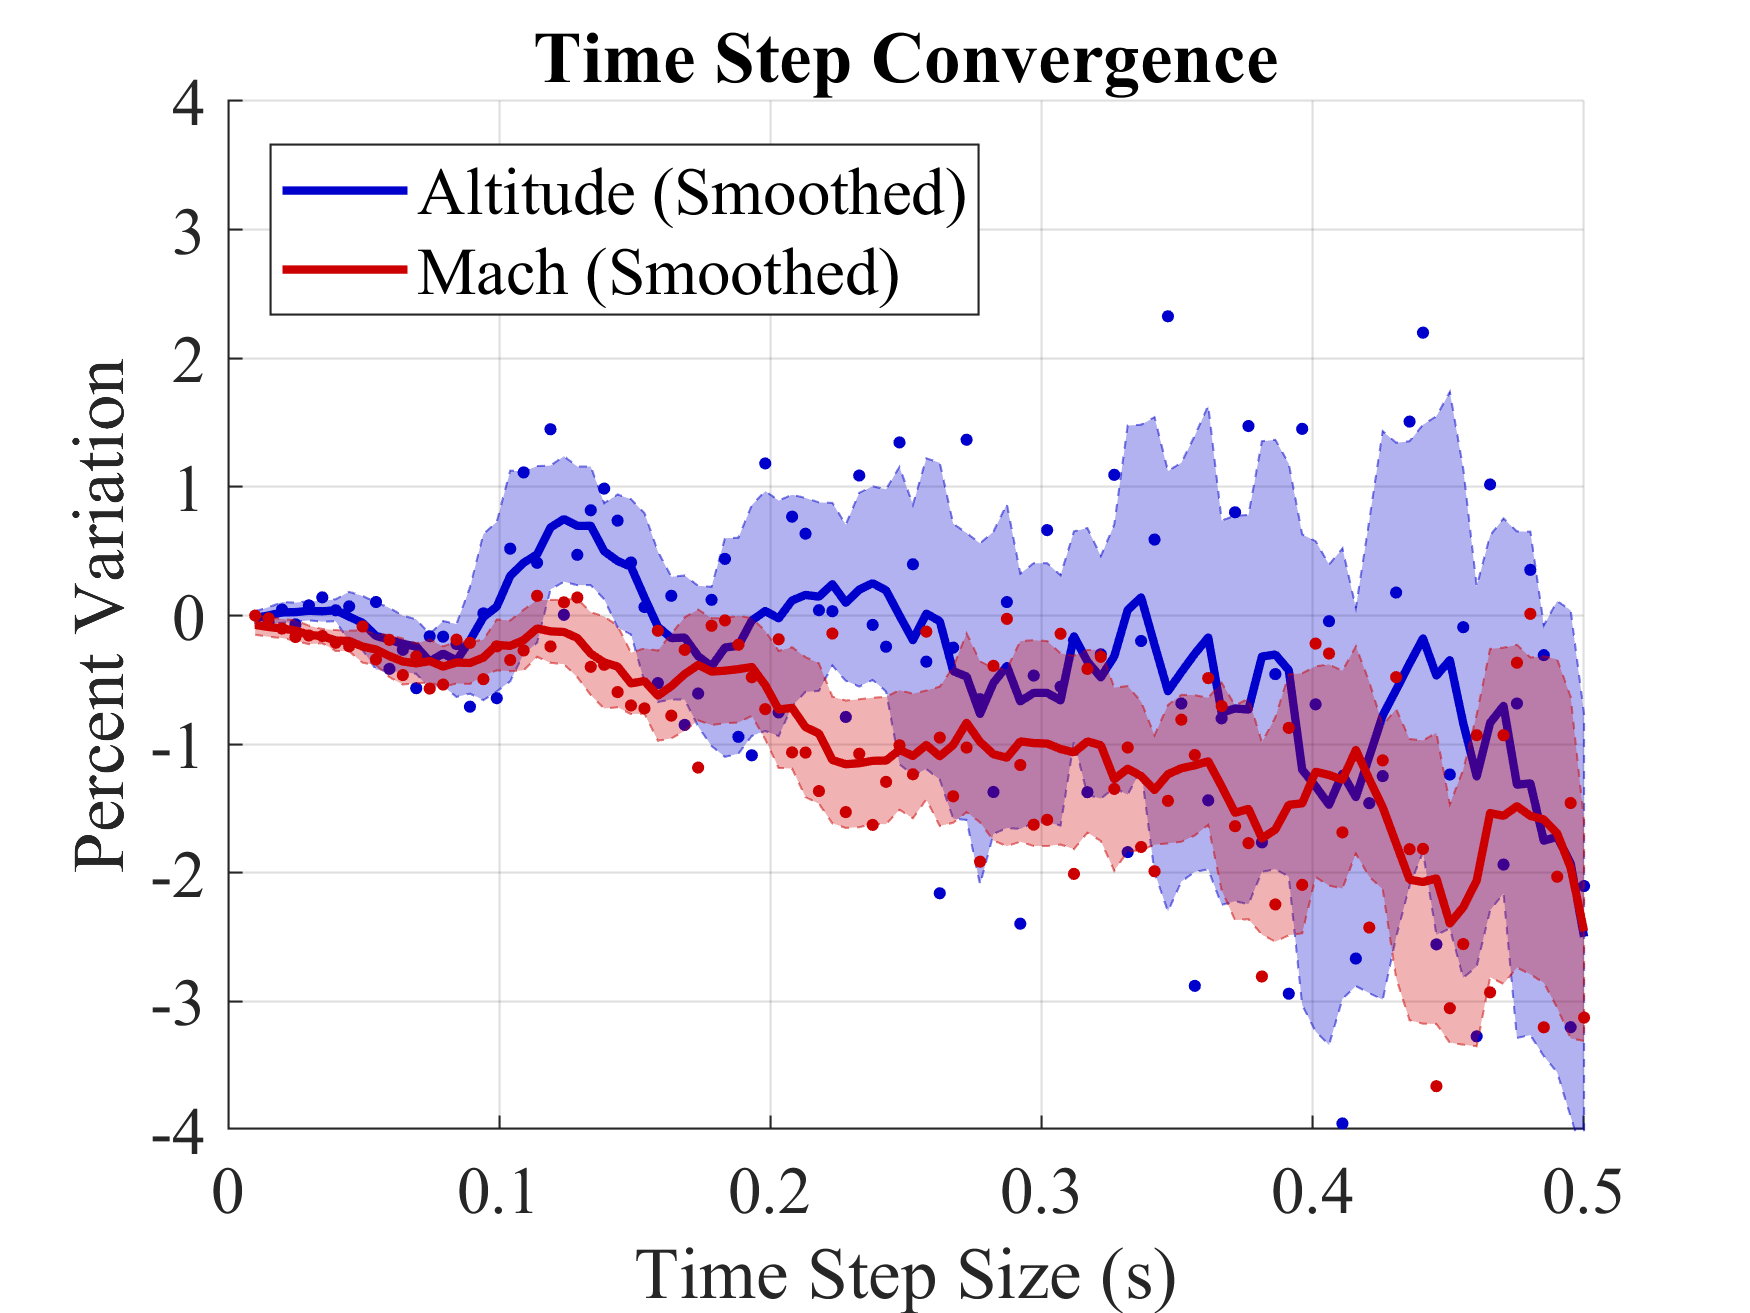
\includegraphics[width=0.75\textwidth]{ModelingAndSim/figures/timeStepConvergence.png}
\caption{Time Step Convergence. Solid lines denote a smoothed mean. Areas show 1$\sigma$ bounds}
\label{fig:timeStepConvergence}
\end{figure}

Results show that variation in Mach and altitude with a different time step sizes is drastically reduces at a time step of less than 0.1 seconds. It is also shown that the variation in Mach and altitude is less than 2 percent for a time step size of 0.25 seconds. For the the purpose this study, a 0.25 second time step will be used to balance computational speed and result quality.

\subsubsection{Control \& Maneuvers}

\paragraph{Launch \& Boost} The orientation of the vehicle during the launch and boost stages was held at a constant elevation angle of 35 degrees. This angle was chosen because it provided a balance between attaining a supersonic drop condition near Mach 2 while setting up the SFRJ stage at and altitude and attitude that made sustained combustion durning subsequent maneuvers feasible. A greater initial angle of attack would tend to drastically increase the final altitude of the SFRJ after its pitch to level flight maneuver, and would also significantly decrease the maximum speed acheived. Lower angles of attack are feasible, but the lower final altitude has its own concerns including increased drag and safety. 

\paragraph{Pitch to Level Flight} After the boost stage burns out and the SFRJ is released, the SFRJ immediately starts burning and pitching down towards level flight. The maneuver was accomplished with a PID controller. The controller was not finely tuned and does exhibit overshoot, but is still effective enough to stabilize the SFRJ. A low integral windup threshold was also implemented to prevent exaggerated and unnecessary overshoot. \color{red}TODO: Controller plots\color{black}

\paragraph{Deflection Maneuvers - Melanie Grande} System-level requirements for the SFRJ included two in-flight maneuvers up to 45\textdegree. Maneuvers are triggered during the SFRJ burn twice, following the pitch to level flight. Conceptually, the SFRJ performs maneuvers by rolling 90-180\textdegree towards the deflection direction, then actuating its fins to effect maximum turn rate. This is implemented in the simulator simply by setting a deflection goal (i.e. 45\textdegree), updating the roll orientation of the vehicle, and tracking the obtained turn over each time step until the deflection is achieved. The simulation is effective, but it could be improved in future work by developing a controller, e.g. PID. 

The SFRJ does manage to complete two deflection maneuvers of 45\textdegree during its burn. Each maneuver takes approximately \color{red}XX seconds\color{black}. Following the maneuvers, the simulation again calls the level flight controller for the remainder of the SFRJ's flight/coast time. 